\documentclass{beamer}
\usepackage{amsmath}
\usepackage[english]{babel} %set language; note: after changing this, you need to delete all auxiliary files to recompile
\usepackage[utf8]{inputenc} %define file encoding; latin1 is the other often used option
\usepackage{csquotes} % provides context sensitive quotation facilities
\usepackage{graphicx} %allows for inserting figures
\usepackage{booktabs} % for table formatting without vertical lines
\usepackage{textcomp} % allow for example using the Euro sign with \texteuro
\usepackage{stackengine}
\usepackage{wasysym}
\usepackage{tikzsymbols}
\usepackage{textcomp}
\newcommand{\bubblethis}[2]{
        \tikz[remember picture,baseline]{\node[anchor=base,inner sep=0,outer sep=0]%
        (#1) {\underline{#1}};\node[overlay,cloud callout,callout relative pointer={(0.2cm,-0.7cm)},%
        aspect=2.5,fill=yellow!90] at ($(#1.north)+(-0.5cm,1.6cm)$) {#2};}%
    }%
\tikzset{face/.style={shape=circle,minimum size=4ex,shading=radial,outer sep=0pt,
        inner color=white!50!yellow,outer color= yellow!70!orange}}
%% Some commands to make the code easier
\newcommand{\emoticon}[1][]{%
  \node[face,#1] (emoticon) {};
  %% The eyes are fixed.
  \draw[fill=white] (-1ex,0ex) ..controls (-0.5ex,0.2ex)and(0.5ex,0.2ex)..
        (1ex,0.0ex) ..controls ( 1.5ex,1.5ex)and( 0.2ex,1.7ex)..
        (0ex,0.4ex) ..controls (-0.2ex,1.7ex)and(-1.5ex,1.5ex)..
        (-1ex,0ex)--cycle;}
\newcommand{\pupils}{
  %% standard pupils
  \fill[shift={(0.5ex,0.5ex)},rotate=80] 
       (0,0) ellipse (0.3ex and 0.15ex);
  \fill[shift={(-0.5ex,0.5ex)},rotate=100] 
       (0,0) ellipse (0.3ex and 0.15ex);}

\newcommand{\emoticonname}[1]{
  \node[below=1ex of emoticon,font=\footnotesize,
        minimum width=4cm]{#1};}
\usepackage{scalerel}
\usetikzlibrary{positioning}
\usepackage{xcolor,amssymb}
\newcommand\dangersignb[1][2ex]{%
  \scaleto{\stackengine{0.3pt}{\scalebox{1.1}[.9]{%
  \color{red}$\blacktriangle$}}{\tiny\bfseries !}{O}{c}{F}{F}{L}}{#1}%
}
\newcommand\dangersignw[1][2ex]{%
  \scaleto{\stackengine{0.3pt}{\scalebox{1.1}[.9]{%
  \color{red}$\blacktriangle$}}{\color{white}\tiny\bfseries !}{O}{c}{F}{F}{L}}{#1}%
}
\usepackage{fontawesome} % Social Icons
\usepackage{epstopdf} % allow embedding eps-figures
\usepackage{tikz} % allows drawing figures
\usepackage{amsmath,amssymb,amsthm} %advanced math facilities
\usepackage{lmodern} %uses font that support italic and bold at the same time
\usepackage{hyperref}
\usepackage{tikz}
\usepackage{tcolorbox}


\usefonttheme[onlymath]{serif} %set math font to serif ones

\definecolor{beamerblue}{rgb}{0.2,0.2,0.7} %define beamerblue color for later use

%%% defines highlight command to set text blue
\newcommand{\highlight}[1]{{\color{blue}{#1}}}


%%%%%%% commands defining backup slides so that frame numbering is correct

\newcommand{\backupbegin}{
   \newcounter{framenumberappendix}
   \setcounter{framenumberappendix}{\value{framenumber}}
}
\newcommand{\backupend}{
   \addtocounter{framenumberappendix}{-\value{framenumber}}
   \addtocounter{framenumber}{\value{framenumberappendix}}
}

%%%% end of defining backup slides

%Specify figure caption, see also http://tex.stackexchange.com/questions/155738/caption-package-not-working-with-beamer
\setbeamertemplate{caption}{\insertcaption} %redefines caption to remove label "Figure".
%\setbeamerfont{caption}{size=\scriptsize,shape=\itshape,series=\bfseries} %sets figure  caption bold and italic and makes it smaller

\newtcolorbox{boxA}{
    fontupper = \bf,
    boxrule = 1.5pt,
    colframe = black % frame color
}


\usetheme{Boadilla}

% --------------------
% Overall information
% --------------------
\title[Economía I]{Economía I \vspace{4mm}
\\ Magistral 20: El Mecano}
\date{}
\author[Riottini]{Riottini Franco}
\vspace{0.4cm}
\institute[]{Universidad de San Andrés}


\begin{document}

\begin{frame}
\titlepage
\centering
Magistral 19


\includegraphics[scale=0.2]{Slides Principios de Economia/Figures/logoUDESA.jpg} 
\end{frame}


\begin{frame}{Empezamos a armar el mecano: oferta y demanda agregada}

    \begin{itemize}
        \item Demanda Agregada \textsc{“El gasto”} \faCartPlus
        \item Oferta Agregada \textsc{"La capacidad productiva”} \faIndustry
    \end{itemize}
    \vspace{3mm}
    
    \centering
\includegraphics[width=5cm]{Slides Principios de Economia/Figures/P17b.png}\

\end{frame}



\begin{frame}{¿Cómo se determina el producto?}

    \begin{itemize}
        \item Para los \textbf{Clásicos} es la capacidad productiva \faCogs:
            \begin{center}
            \begin{tcolorbox}[width=2in,
                  interior hidden,
                  boxsep=0pt,
                  left=0pt,
                  right=0pt,
                  top=2pt,
                  ]%%
                    $$ \bar{Y}=f(K, L) $$
             \end{tcolorbox}
             \end{center}
             
            \begin{itemize}
            \item El mercado de trabajo determina el empleo
            \item Se produce el PBI "potencial"
              \item "Ley de Say" (la oferta encuentra su demanda)
            \end{itemize}
        
        \item Para los \textbf{Keynesianos} es la demanda \faShoppingBasket:
            
            \begin{center}
            \begin{tcolorbox}[width=2in,
                  interior hidden,
                  boxsep=0pt,
                  left=0pt,
                  right=0pt,
                  top=2pt,
                  ]%%
                    $$ Y = C + I + G $$
             \end{tcolorbox}
             \end{center}
             
            \begin{itemize}
            \item El producto lo determina la demanda agregada
            \item ...si la demanda se ubica por debajo de la capacidad productiva de una economía
            \end{itemize}
    \end{itemize}

\end{frame}


\begin{frame}{Agregamos el mercado de dinero y crédito}

    \begin{itemize}
        \item \textbf{Mercado de Dinero} \faMoney:
            \begin{itemize}
            \item Demanda de Dinero
            
            \begin{center}
            \begin{tcolorbox}[width=1.5in,
                  interior hidden,
                  boxsep=0pt,
                  left=0pt,
                  right=0pt,
                  top=0pt,
                  ]%%
                    $$ L_{d}=f(Y, i, P) $$
             \end{tcolorbox}
             \end{center}
            
            \item Oferta de Dinero (multiplicador monetario)
            \item Según los supuestos este mercado determina o los precios o la tasa de interés
            \end{itemize}
        
        \item \textbf{Mercado de Crédito} \faBank:
            \begin{itemize}
             \item Demanda de Crédito
                \begin{itemize}
                \item Deuda pública + Inversión
                \end{itemize}
              \item Oferta de Crédito
                \begin{itemize}
                \item Ahorro interno y externo

            \begin{center}
            \begin{tcolorbox}[width=2in, boxsep=0pt, left=0pt, right=0pt, top=0pt,]%%
                    $$ \Delta D+I=A_{i}+A_{e x t} $$
             \end{tcolorbox}
             \end{center}
                \end{itemize}
            \item Este mercado determina o la tasa de interés real o la demanda agregada
            \end{itemize}
    \end{itemize}

\end{frame}



\begin{frame}{Esta sería la secuencia de causalidad}

\centering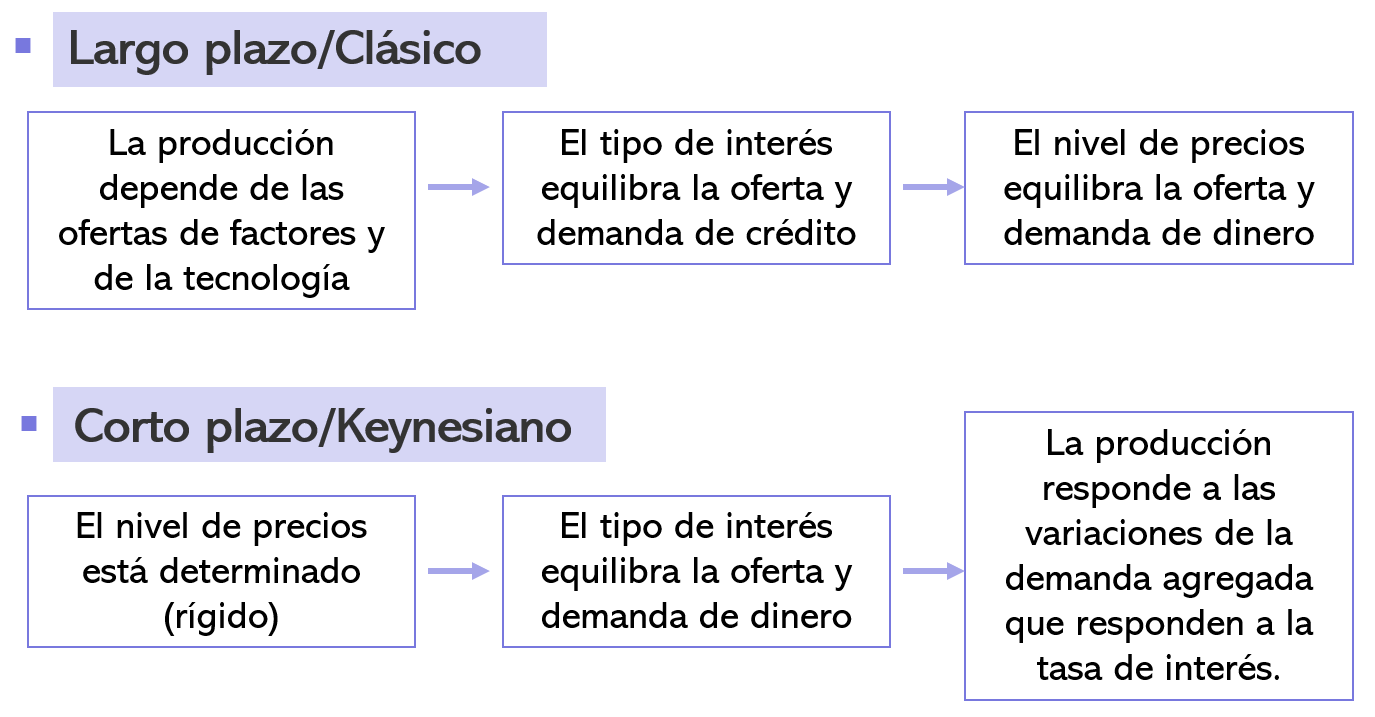
\includegraphics[width=11cm]{Slides Principios de Economia/Figures/P18.png}\

\end{frame}


\begin{frame}{El enfoque Clásico y Keynesiano: Oferta Agregada}

\begin{itemize}
        \footnotesize\item La curva OA relaciona P (precios) con Y (producto).
        \footnotesize\item La forma de esta curva determina el mercado de trabajo.
\end{itemize}
\vspace{3mm}
\centering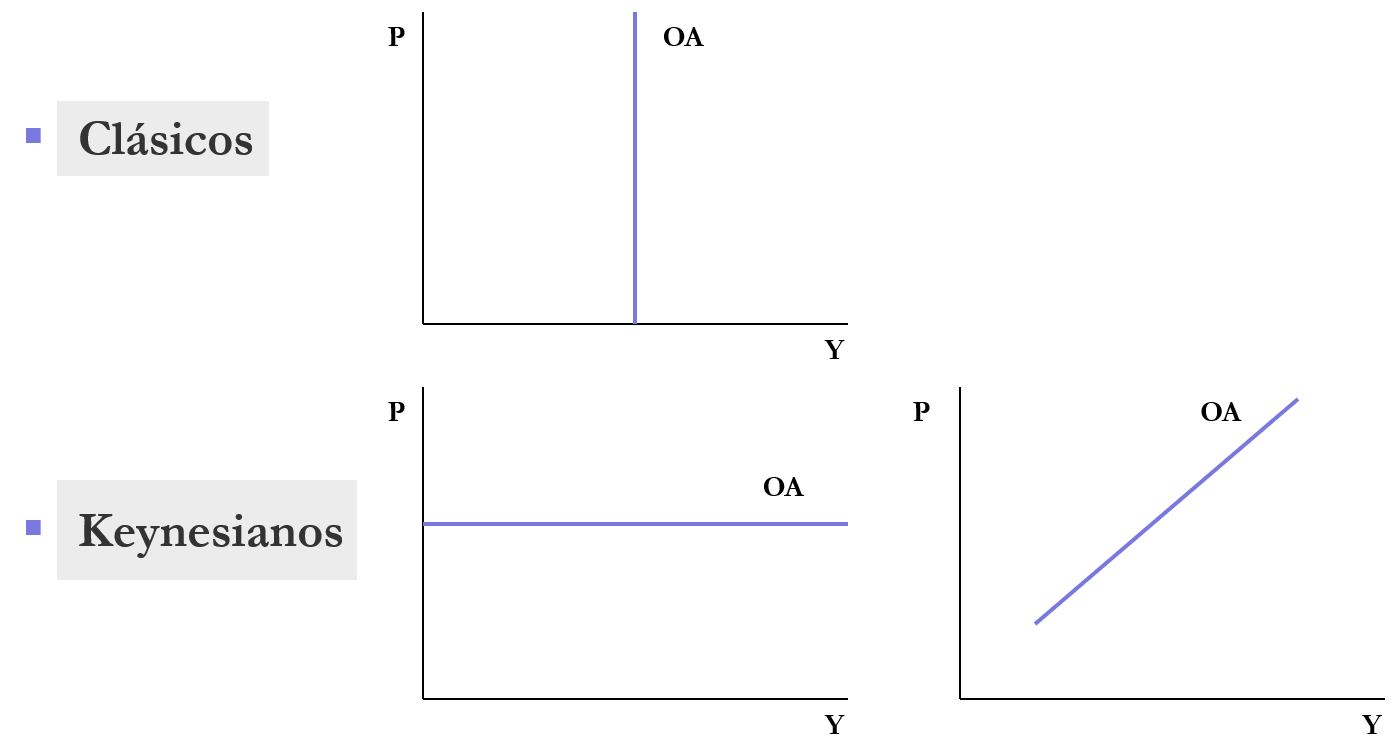
\includegraphics[width=10.5cm]{Slides Principios de Economia/Figures/P19.png}\

\end{frame}


\begin{frame}{El enfoque Clásico y Keynesiano: Demanda Agregada}

\centering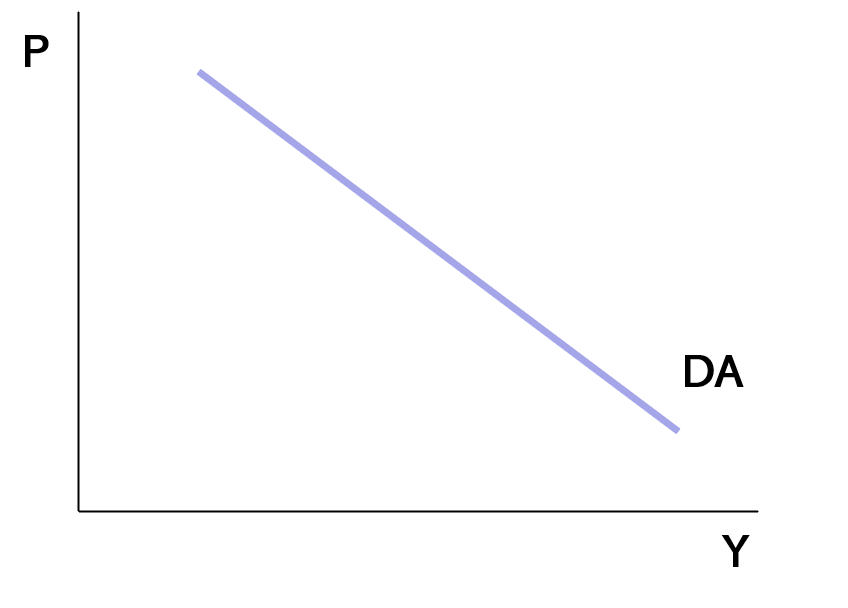
\includegraphics[width=6cm]{Slides Principios de Economia/Figures/P20.png}\

    \begin{itemize}
        \item La forma de esta curva determina como C (consumo) e I (inversión) reaccionan frente al nivel de P (precios)
        \item El consumo y la inversión caen debido al incremento en los precios:
            \begin{itemize}
                \item Efecto riqueza
                \item Efecto tasa de interés: un aumento de P sin cambiar M lleva a tasas de interés más altas que hacen caer C e I.
            \end{itemize}
    \end{itemize}

\end{frame}



\begin{frame}{Shocks a la Demanda Agregada}
    
\centering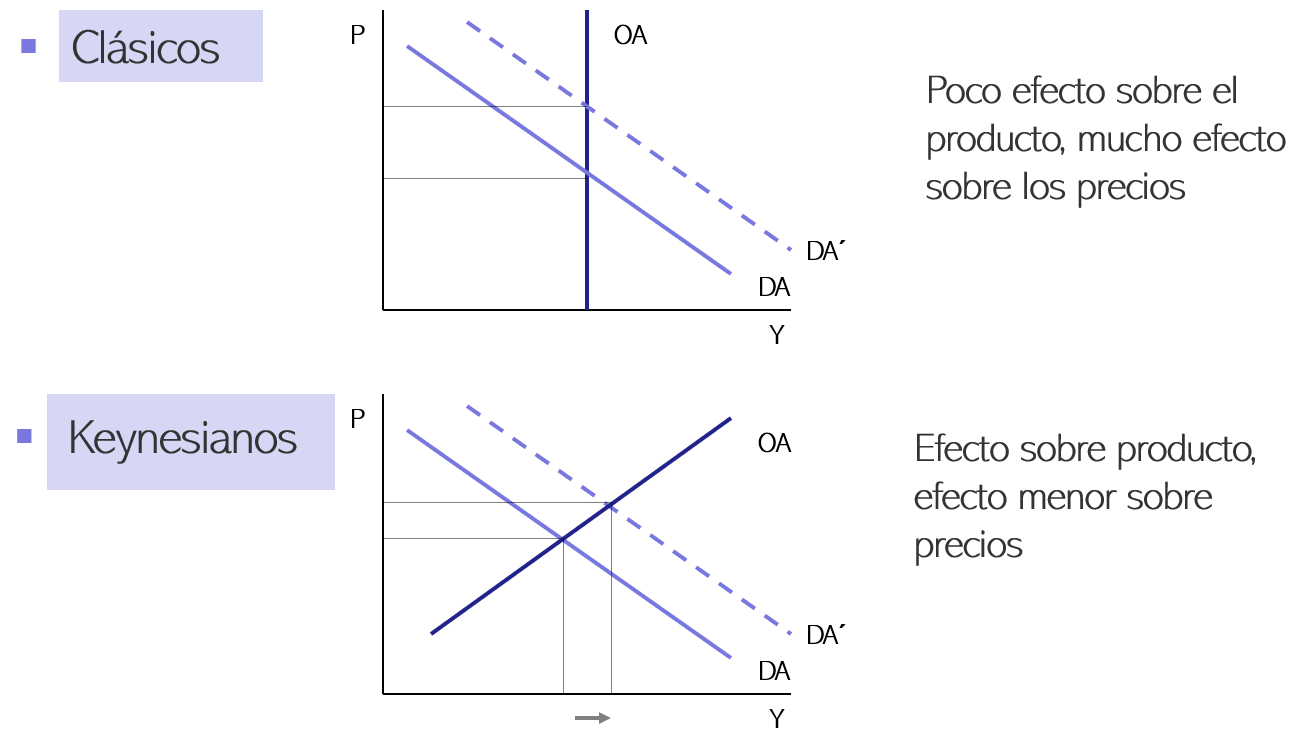
\includegraphics[width=11cm]{Slides Principios de Economia/Figures/P21.png}\
    
\end{frame}


\begin{frame}{Shocks a la Oferta Agregada}

Los shocks de oferta negativos  producen un fenómeno que se conoce como estanflación

\begin{figure} [H]
\centering
\begin{minipage}{.5\textwidth}
  \centering
  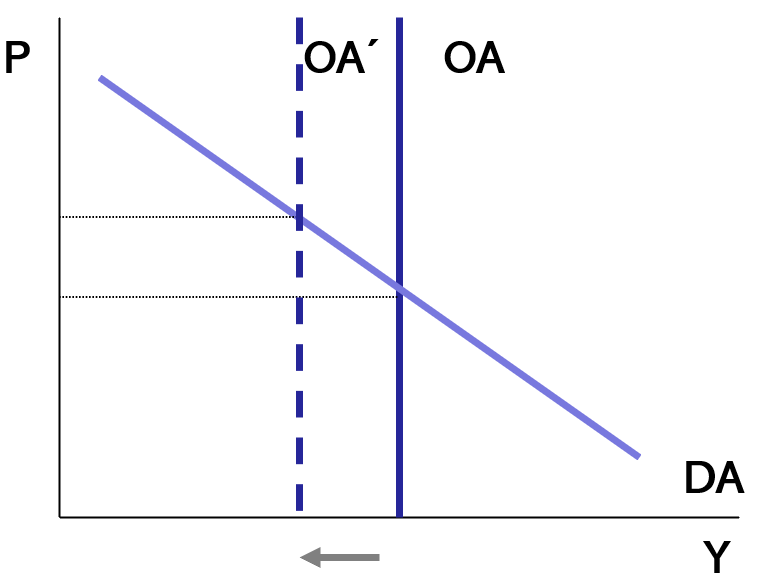
\includegraphics[width=0.9\textwidth]{Slides Principios de Economia/Figures/P22_1.png}
  \caption{\textbf{Clásicos}}
  \label{a}
\end{minipage}%
\begin{minipage}{.5\textwidth}
  \centering
  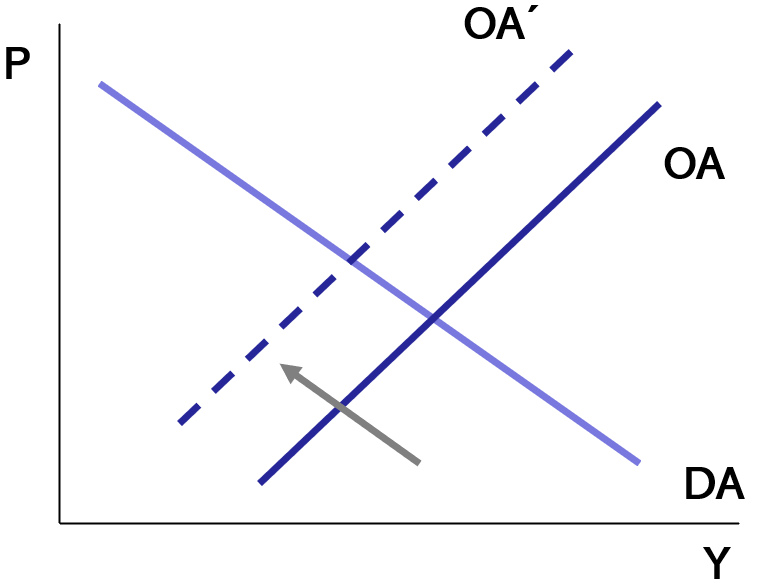
\includegraphics[width=0.9\textwidth]{Slides Principios de Economia/Figures/P22_2.png}
  \caption{\textbf{Keynesianos}}
  \label{b}
\end{minipage}
\\
\end{figure}
\end{frame}




\begin{frame}{Ciclos: los Clásicos}

\begin{itemize}
    \item La explicación clásica de las fluctuaciones viene por cambios en la oferta agregada
\end{itemize}

\vspace{2mm}
 
\begin{center}
\begin{figure}[H]
\renewcommand{\figurename}{Figure}
\begin{center}
    \begin{minipage}[b]{0.45\textwidth}
        \begin{center}
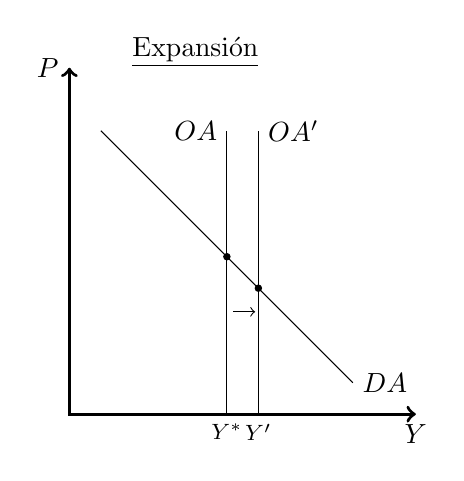
\begin{tikzpicture}[scale=0.4]
\draw[very thick,<->] (0,11) node[left]{$P$}--(0,0)--(11,0) node[below]{$Y$};
\draw[thin](6,0)--(6,9) node [right] {$OA'$};
\draw[thin](5,0)--(5,9) node [left] {$OA$};
\draw[thin](1,9)--(9,1) node [right] {$DA$};
\draw[thin, ->] (5.2,3.25)--(5.9,3.25);
\node[below] at (5,0) {\footnotesize $Y^{*}$};
\node[below] at (6,0) {\footnotesize $Y'$};
\draw[fill](5,5) circle [radius =0.1];
\draw[fill](6,4) circle [radius =0.1];
\node[] at(4,11.5) {\underline{Expansión}};
\end{tikzpicture}
\end{center}
     \end{minipage}
  %  \hfill
    \begin{minipage}[b]{0.45\textwidth}
    \begin{center}
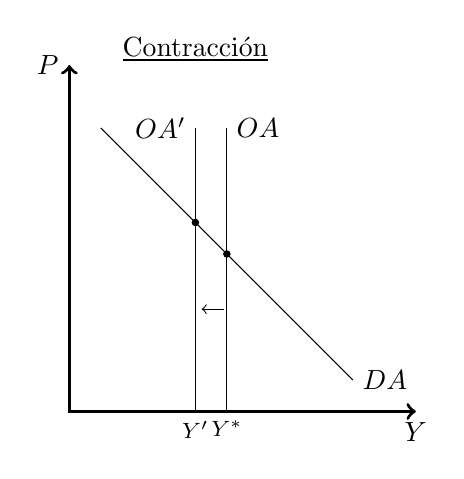
\begin{tikzpicture}[scale=0.4]
\draw[very thick,<->] (0,11) node[left]{$P$}--(0,0)--(11,0) node[below]{$Y$};
\draw[thin](5,0)--(5,9) node [right] {$OA$};
\draw[thin](4,0)--(4,9) node [left] {$OA'$};
\draw[thin](1,9)--(9,1) node [right] {$DA$};
\draw[thin, ->] (4.9,3.25)--(4.2,3.25);
\node[below] at (5,0) {\footnotesize $Y^{*}$};
\node[below] at (4,0) {\footnotesize $Y'$};
\draw[fill](5,5) circle [radius =0.1];
\draw[fill](4,6) circle [radius =0.1];
\node[] at(4,11.5) {\underline{Contracción}};
\end{tikzpicture}
\end{center}
    \end{minipage}
\end{center}
\end{figure}
\end{center} 
\end{frame}



\begin{frame}{Ciclos: los Keynesianos}

\begin{itemize}
    \item La explicación keynesiana de las fluctuaciones viene por cambios en la demanda agregada
\end{itemize}

\vspace{2mm}

\begin{center}
\begin{figure}[H]
\renewcommand{\figurename}{Figure}
\begin{center}
    \begin{minipage}[b]{0.45\textwidth}
        \begin{center}
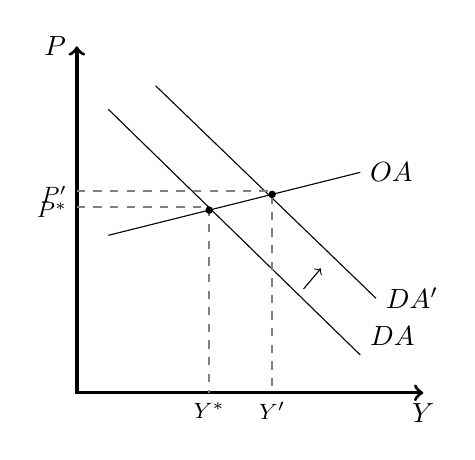
\begin{tikzpicture}[scale=0.4]
\draw[very thick,<->] (0,11) node[left]{$P$}--(0,0)--(11,0) node[below]{$Y$};
\draw[thin](1,5)--(9,7) node [right] {$OA$};
\draw[thin](1,9)--(9,1.2) node [above right] {$DA$};
\draw[thin](2.5,9.75)--(9.5,3) node [right] {$DA'$};
\draw[thin, <-] (7.75,3.95)--(7.2,3.3);
\draw[thick,gray,dashed](0, 6.4)--(6.2, 6.4)--(6.2, 0);
\draw[thick,gray,dashed](0,5.9)--(4.2,5.9)--(4.2, 0);
\node[left] at (0,5.8) {\footnotesize $P^{*}$};
\node[left] at (0,6.3) {\footnotesize $P'$};
\node[below] at (6.2,0) {\footnotesize $Y'$};
\node[below] at (4.2,0) {\footnotesize $Y^{*}$};
\draw[fill](6.2,6.3) circle [radius =0.1];
\draw[fill](4.2,5.8) circle [radius =0.1];
\end{tikzpicture}
\end{center}
     \end{minipage}
  %  \hfill
    \begin{minipage}[b]{0.45\textwidth}
    \begin{center}
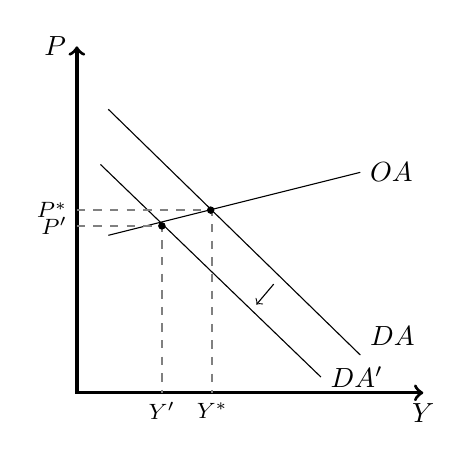
\begin{tikzpicture}[scale=0.4]
\draw[very thick,<->] (0,11) node[left]{$P$}--(0,0)--(11,0) node[below]{$Y$};
\draw[thin](1,5)--(9,7) node [right] {$OA$};
\draw[thin](1,9)--(9,1.2) node [above right] {$DA$};
\draw[thin](0.75,7.25)--(7.75,0.5) node [right] {$DA'$};
\draw[thin, ->] (6.25,3.45)--(5.7,2.8);
\draw[thick,gray,dashed](0, 5.3)--(2.7,5.3)--(2.7, 0);
\draw[thick,gray,dashed](0,5.8)--(4.3,5.8)--(4.3, 0);
\node[left] at (0,5.3) {\footnotesize $P'$};
\node[left] at (0,5.8) {\footnotesize $P^{*}$};
\node[below] at (4.3,0) {\footnotesize $Y^{*}$};
\node[below] at (2.7,0) {\footnotesize $Y'$};
\draw[fill](2.7,5.3) circle [radius =0.1];
\draw[fill](4.25,5.8) circle [radius =0.1];
\end{tikzpicture}
\end{center}
    \end{minipage}
\end{center}
\end{figure}
\end{center} 
\end{frame}


%---------------------------------------------------------------------------%
%---------------------------------------------------------------------------%

%\begin{frame}{}
%\centering 	\huge \textbf{El mercado de trabajo y la oferta %agregada} 
%\vspace{2mm}
%\hrule
%\end{frame}
%---------------------------------------------------------------------------%
%---------------------------------------------------------------------------%

%---------------------------------------------------------------------------%






\end{document}